\documentclass[a4paper,12pt]{report}

\usepackage{alltt, fancyvrb, url}
\usepackage{graphicx}
\usepackage[utf8]{inputenc}
\usepackage{float}
\usepackage{hyperref}


\title{OOP Java project \\Budmate:\\ Personal budget manager}

\author{
    alessandro.stefani10@studio.unibo.it \\
    giulio.salotti@studio.unibo.it \\
    paolo.pietrelli@studio.unibo.it \\
    zhaohui.song@studio.unibo.it
}

\date{\today}

\begin{document}

\maketitle

\tableofcontents

\chapter{Analisi}

\section{Requisiti}

In the year 2022 due to the federal reserve's decision, a lot of liquidity floods into the market, many people are lured in to make some bucks.
But the market is like an ocean, teeming with volatilities. 
Though various platforms have emerged, we lacked a tool to manage every income and expenditure, our idea is to build a cloud-based platform that connects to various markets, provides analysis tools to clients to minimize the risk, and get the big picture of actual assets. .
It's a tiny project of about 80 hours amount of work, hence it will only be a prototype.
\\
This software was supposed to provide visual tools to analyze market conditions, but it will be implemented once all basic functionalities are satisfied.
%
Such as using deep learning to analyze future accounts' conditions based on the historic data. (Backtracking).

\subsection*{Elementi positivi}
\begin{itemize}
    \item The software should be able to manage various assets of a client.
    \item management of one or more profiles including registration and switching between accounts.
    \item account management, piggy banks, investment management, and expense management.
    \item vision of the stock and crypto markets.
\end{itemize}

\subsection*{Elementi negativi}
\begin{itemize}
    \item This software depends on if a platform such as \textit{Binance} \footnote{\url{https://www.binance.com/en/binance-api}} gives an open API, then your action on the budmate will actually be executed on the Binance platform.
\end{itemize}


\subsubsection{Requisiti funzionali}
\begin{itemize}
    \item There should be a login and registration screen upon software's activation, authentication of profile via database or google / Facebook authenticator.
    \item A profile page contains everything about the user, including total value, number of accounts, activities, subscription plan, whether the client needs to pay fees or not, and even accessing friends' pages.
    \item Investment page: an over\textit{view} of all assets owned on various platforms, a chart showing the trend of the total value of the investments. The ability to purchase and sell assets, such as BITCOIN, and APPLE. In the future, there will also be NFT markets, government bonds, real estate, and maybe even gaming assets(metaverse).
    \item Accounts page: Bank accounts, investment accounts, Budmate accounts, with various information containing IBAN, and swift code. 
    The ability to create or connect to an existing bank account, whether is Uni credit or Goldman Sachs.
    \item Expenditure page:  shows various kinds of expenses done in the shopping mall, grocery store, book shop, restaurants, cafe bar, monthly subscriptions, student loans, and charts with visual future trends.
\end{itemize}

\subsubsection{Requisiti non funzionali}
\begin{itemize}
    \item For the workflow, we use git and develop the software on different machines and OS, including windows, ubuntu 22.04, 20.04, and macOS. 
    \item The architecture of software should be highly independent, If one member couldn't work full time, that shouldn't bother the others' work.
\end{itemize}

\section{Analisi e modello del dominio}
Our app starts from the profile class, in the profile, there can be many types of accounts: 
such as expenses, bank accounts, investment accounts, holding accounts, and even Budmate accounts. Those accounts have similar functionalities, in below, you can find specific implementations.

\subsection*{Elementi positivi}
\begin{itemize}
    \item easy structure, simple responsibility.
    \item independent implementation without depending on the other's realization, the use of interface.
\end{itemize}

\subsection*{Elementi negativi}
\begin{itemize}
    \item Its functionality is dependent on access to the internet, If a user is offline, it's hard to do any trading operation.
\end{itemize}


\begin{figure}[H]
\centering{}
\makebox[\textwidth][c]{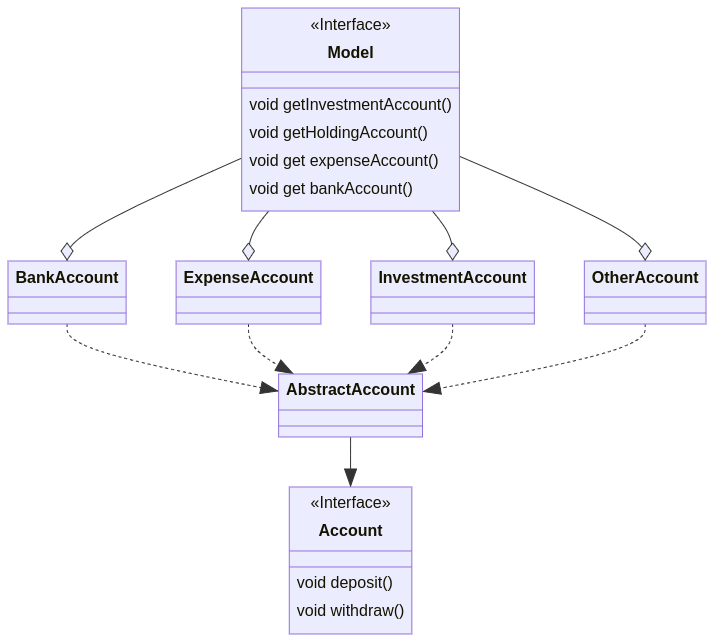
\includegraphics[width=1.2\textwidth]{img/domainAnalysis.png}}%
\caption{Our structure of model}
\label{img:domainAnalysis}
\end{figure}

\chapter{Design}
Our design fulfills tremendously \textit{5 design principles}
\subsection*{principles}
\begin{itemize}
    \item DRY: Don’t repeat yourself 
    \item KISS: Keep it simple, stupid 
    \item SRP: Single Responsibility Principle
    \item OCP: Open-clodes principle
    \item DIP: Dependency-inversion principle
\end{itemize}

\section{Architettura}
    We use design pattern MVC(\textit{view}, control, model) for our whole structure, we use JavaFX for our \textit{view} and other \textit{view}s for logging.  
    A controller that gets notified by JavaFX event, access model for computation then updates the \textit{view}.  

\subsection*{Elementi positivi}
\begin{itemize}
    \item By using MVC and Interface, we can switch between JavaFX and other graphic libraries without changing other parts. 
    \item We use other threads to compute tasks that uses a lot of time.
\end{itemize}


\begin{figure}[H]
    \centering{}
    \makebox[\textwidth][c]{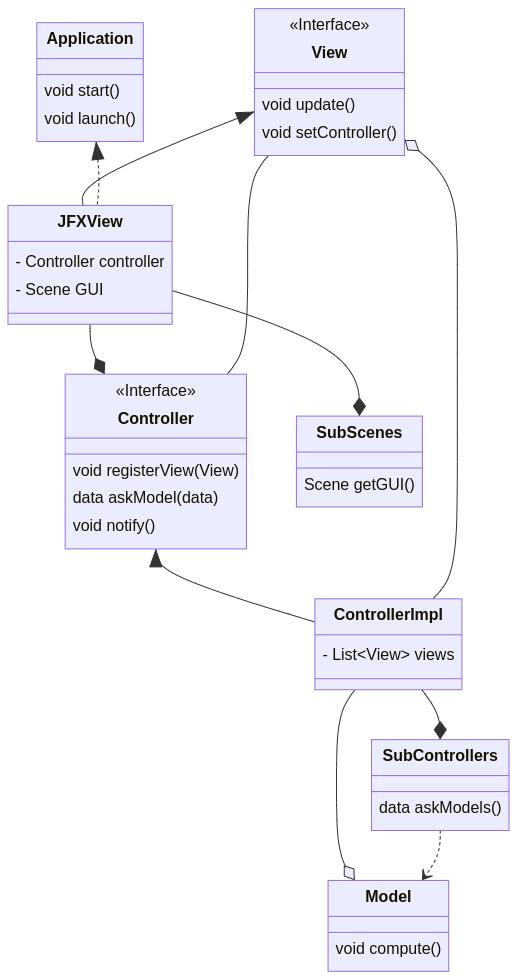
\includegraphics[width=0.75\textwidth]{img/MVC.png}}%
    \caption{Our structure of MVC implementation}
    \label{img:MVC}
    \end{figure}

%%\Cref{img:} è esemplificato il diagramma UML architetturale.


\section{Design dettagliato}

\subsection{Zhaohui Song}

Since I started the project earlier than the others, I feel that I don't want the others to rewrite the same piece of code multiple times, so every design should at least satisfy DRY OCP, either for the Model or the GUI.
%
\\\\Some patterns are perfectly fit for my solution including the \textit{Factory method, Builder, Template method, Iterator, Strategy, Observer, and Decorato}r, I avoided \textit{singleton} as much as possible.
%
\\\\Some functions are left open because as mentioned above, we may need to add the third-party API to fulfill the order done by the client. Like if a user Bob wants to buy a share of Amazon stock since our app is a kind of portfolio tracker,  
he can hit the button Buy in our app, then our app will send the order to the actual broker app, the advantage is you can analyze the data using our app, then executing the order automatically to various platform, in the case one platform bankrupts, you won't lose everything.
%
\\\\You may not see all implementations of these functionalities, but I think when it comes to design an app, I ought to make it equipped with  \textbf{scalability,  interoperability}(coherent with other existing apps, because I don't want to write something that already exists), \textbf{standardized, feature-complete, and easy for the rest of team members to develop}.
And by thinking that, I used most of my 80 hours to make it easier for the others use.
%
\subsubsection{Generalise Account as much as possible and create my part InvestmentAccount}
\begin{figure}[H]
    \centering{}
    \makebox[\textwidth][c]{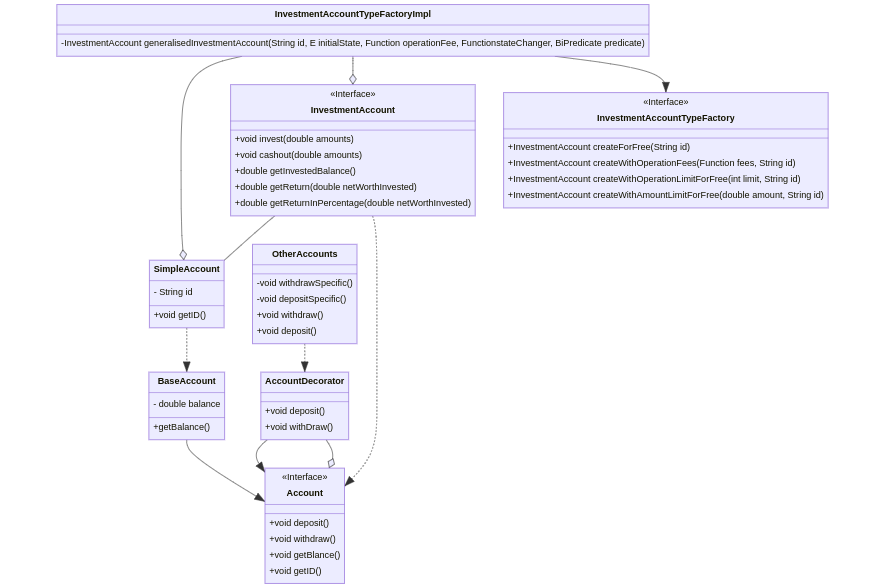
\includegraphics[width=1.7\textwidth]{img/invAccount.png}}%
    \caption{generalised Account}
    \label{img:invAccount}
    \end{figure}

    \paragraph{Problem:} Make an account interface that's common to everybody

    \paragraph{Solution:} An interface that satisfies basic operations such as deposit and withdrawal. In my opinion, all accounts are basically simple accounts, So you can either extend it to make a more detailed realization or implement \textbf{\textit{decorators}} to add single responsibilities to the easy account, or even use it as a component as I did in my investment account factory.
    %
    \\ \textbf{Note}: The decorator here is not implemented, because it was designed for open changes. As an example, if someone wants to add a layered fee based on the accounts' features or traits, one can simply create an account using a new AccountWithFeePlanPlatinium(new Account) without the necessity of using the factory method.

    \paragraph*{Problem:} When this app is ready, I need to think about how to make a profit, depends on the current user's description plan, we may charge a fee to his trading operation, add a limit to the number of times that a user can trade, and add the limit amount for withdrawal, etc. 

    \paragraph*{Solution:} As I will have multiple genres of investment Accounts, I create a factory that builds different investment accounts for me. Here I used \textbf{strategy}(function and bipredicate) via lambda expression for how to charge a fee form client;
    An initial state with a generic type to define based on what factor a limit can be added. The pattern used here consists of the \textbf{Factory method, template method}. 


\subsubsection*{Need a place to trade stocks with the real-time price change}
    \begin{figure}[H]
    \centering{}
    \makebox[\textwidth][c]{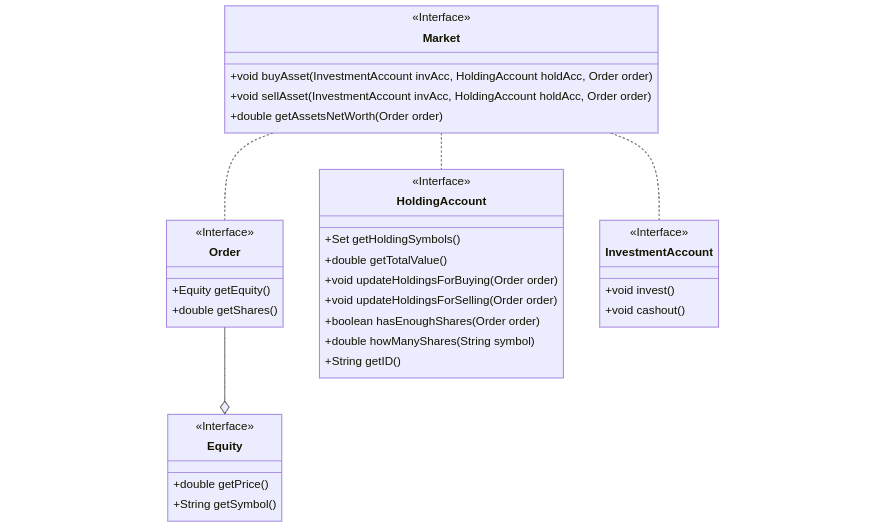
\includegraphics[width=1.3\textwidth]{img/market.png}}%
    \caption{market}
    \label{img:market}
    \end{figure}

    \paragraph{Problem:} How to trade generalised assets with real-time prices

    \paragraph*{Solution:} Here I generalize every kind of asset into class Equity, which can be either stock, cryptos, NFTs, commodities, ETFs, etc. All we need is a symbol and its price. As you see in the figure above, when a user trade with a symbol, assets will be added to the holding account, and money will be decreased in the corresponding investment account.

\subsubsection*{A group of databases to retrieve real world information}
\begin{figure}[H]
    \centering{}
    \makebox[\textwidth][c]{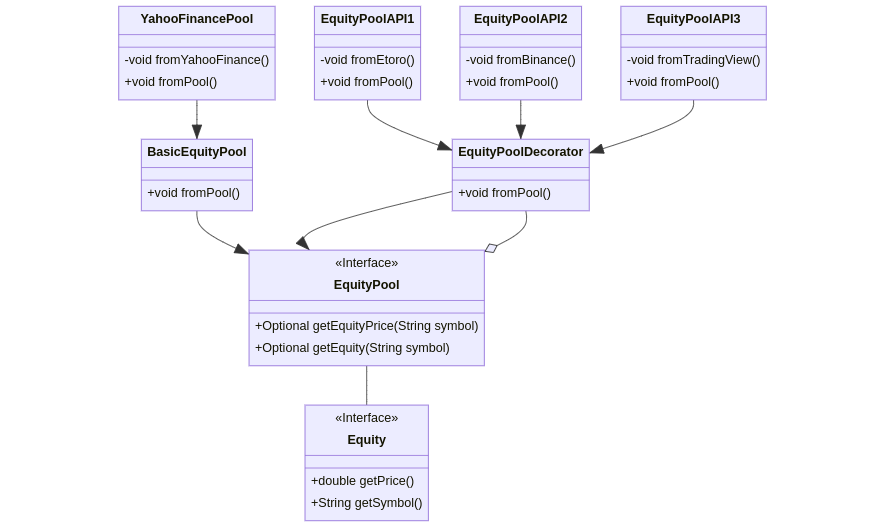
\includegraphics[width=1.3\textwidth]{img/EquityPool.png}}%
    \caption{EquityPool}
    \label{img:EquityPool}
    \end{figure}

    \paragraph{Problem:} How to query prices from more platforms

    \paragraph*{Solution:}Using the design pattern \textbf{decorator} perfectly resolved this problem, firstly we search the price on our default platform Yahoo Finance. In the case we know that an asset may not be found there, we can add more layers for searching from other platforms. It's like a cache hit(how the CPU uses cache to find data in the memory). If the price can be found in the cache of level 1, then that's it, otherwise, it will searches from the cache level 2...n till the central memory. 
    As an example, if a user were searching for a 10-year government bond, it's likely that it won't appear in the market. Then we can do Equity eq = new EquityPoolApiBond(new YahooFinancePool());  So we cover the searching as much as possible.

\subsubsection*{Abstracting javafx from the \textit{view}}
\begin{figure}[H]
    \centering{}
    \makebox[\textwidth][c]{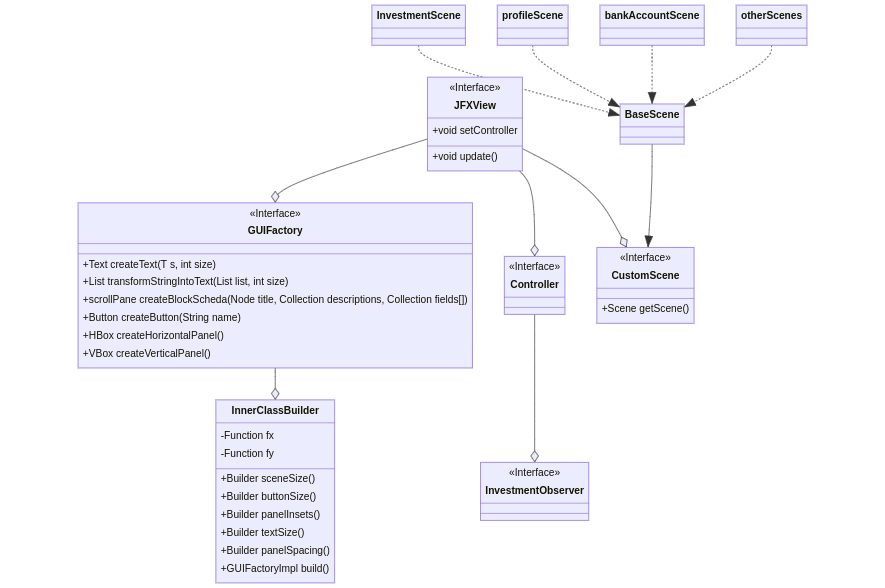
\includegraphics[width=1.3\textwidth]{img/observer.png}}%
    \caption{Observer for \textit{view}s with multithreading}
    \label{img:Observer}
    \end{figure}

    \paragraph{Problem:} I spent time on learning JavaFX, how to avoid it for the others

    \paragraph*{Solution:} Gathering all JavaFX creations inside of one class \textit{GUIFactory} is extremely easy for everyone, whoever needs a component, can be created using a factory class without tedious settings. I used an inner class Builder to set configurations. In this design, every element's size of the GUI is in the percentage of the current screen. So no matter whether you open the app on a 1080p laptop or 8k curved monitor, it's should be always legitimate to read.


    \paragraph{Problem:} Everyone needs to create their own scene, how to avoid everyone working on the same files.

    \paragraph*{Solution:}I created a common class Custom Scene, its attached controller, and main stage, so each member can write its counterpart scene in their class without losing the flexibility of MVC.

    \paragraph{Problem:}Some tasks such as reading data from databases can take a lot of time

    \paragraph*{Solution:}By introducing Task in the controller, some tasks can be done in other background thread,  GUI changes on the JavaFX thread, computational works on background threads, and main app on the main thread. 

    \paragraph{Problem:}Every time a new task emerges, a new thread is being created, how to avoid thread throttling?

    \paragraph*{Solution:}By using ExecutorService we create 10 threads at first, then every task will only be executed on these specified threads, so to avoid throttling

    \paragraph{Problem:}How to convert all kinds of data into Text with the defined format for display.

    \paragraph*{Solution:}In the class of \textit{GUIFactory}, there is a function/algorithm, that accepts arbitrary data type and converts it into String, by using the technique of Reflection in java.

    \paragraph{Problem:}How to update the  widgets with infinite arguments with each of them a different type

    \paragraph*{Solution:} Every time when controller updates a widget on the \textit{\textit{view}}, instead of passing tons of arguments, a \textit{Queue(List(?)) packet} can be used. The merit is you can get an iterator from that, and get infinite of arguments with the arbitrary data type. 

    \subsection*{Elementi positivi}

    \begin{itemize}
        \item  By using design pattern, it easily solved most of the problems
        \item Every piece of code is reusable 
        \item A lot of use of Interface that satisfies Dependency-inversion principle
    \end{itemize}
    
    \subsection*{Elementi negativi}
    \begin{itemize}
        \item In order to be flexible and reusable, each piece of code might be a bit difficult for the others to understand, especially for those who didn't understand OOP concepts.
        \item I've done every class beforehand, but without immediate feedback, I couldn't understand other team member's real needs. 
        \item Since I keep improving my code, there were lots of changes every time I push the code to git, but I still tried to do my best.
    \end{itemize}
    
\subsection{Alessandro Stefani}

    \subsubsection{Profile}
        \paragraph{Problem:}We needed a class to contain all the information about the user, which comprehend both economical and credentials information.
        \paragraph{Solution:}I implemented two simple classes that are able to store, give or update those information when needed by the different Account implementations.
            \begin{figure}[H]
                \centering{}
                \makebox[\textwidth][c]{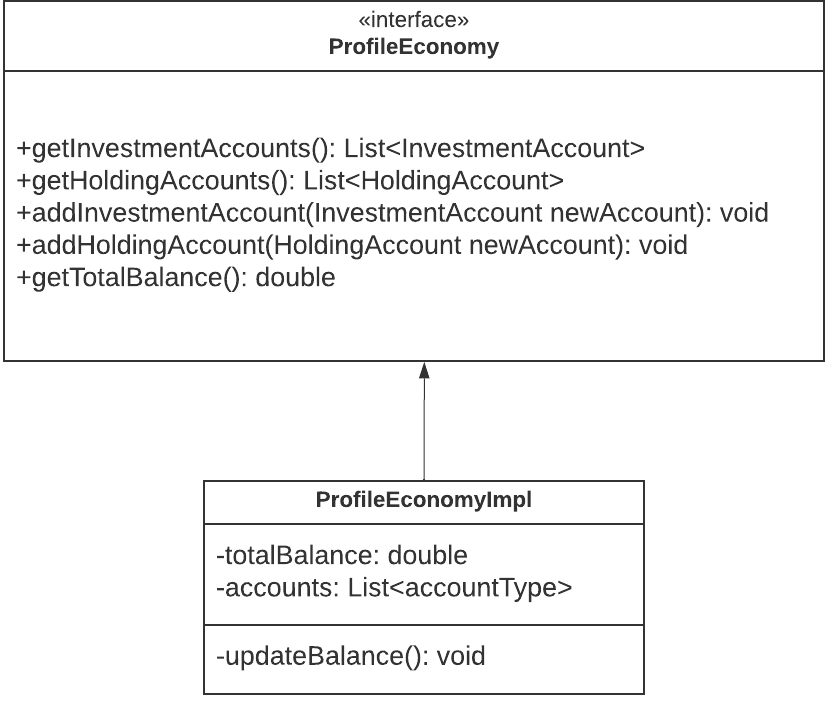
\includegraphics[width=0.8\textwidth]{img/UMLProfileEconomy.png}}%
                \caption{Profile Economy}
                \label{img:my_label}
            \end{figure}
        \paragraph{Note:}The class which stores the user credentials would have been useful for retrieving all user information from a JSON database that was unfortunately not implemented due to a bug.
        
    \subsubsection{Password Change}
        \paragraph{Problem:}While implementing the user profile, i wanted to allow password changes using different "authentications".
        \paragraph{Solution:}Since the algorithm to change password is almost always the same, and only differs on the authentication check, I used strategy to be able to change the behavior of PasswordChanger runtime.
            \begin{figure}[H]
                \makebox[\textwidth][c]{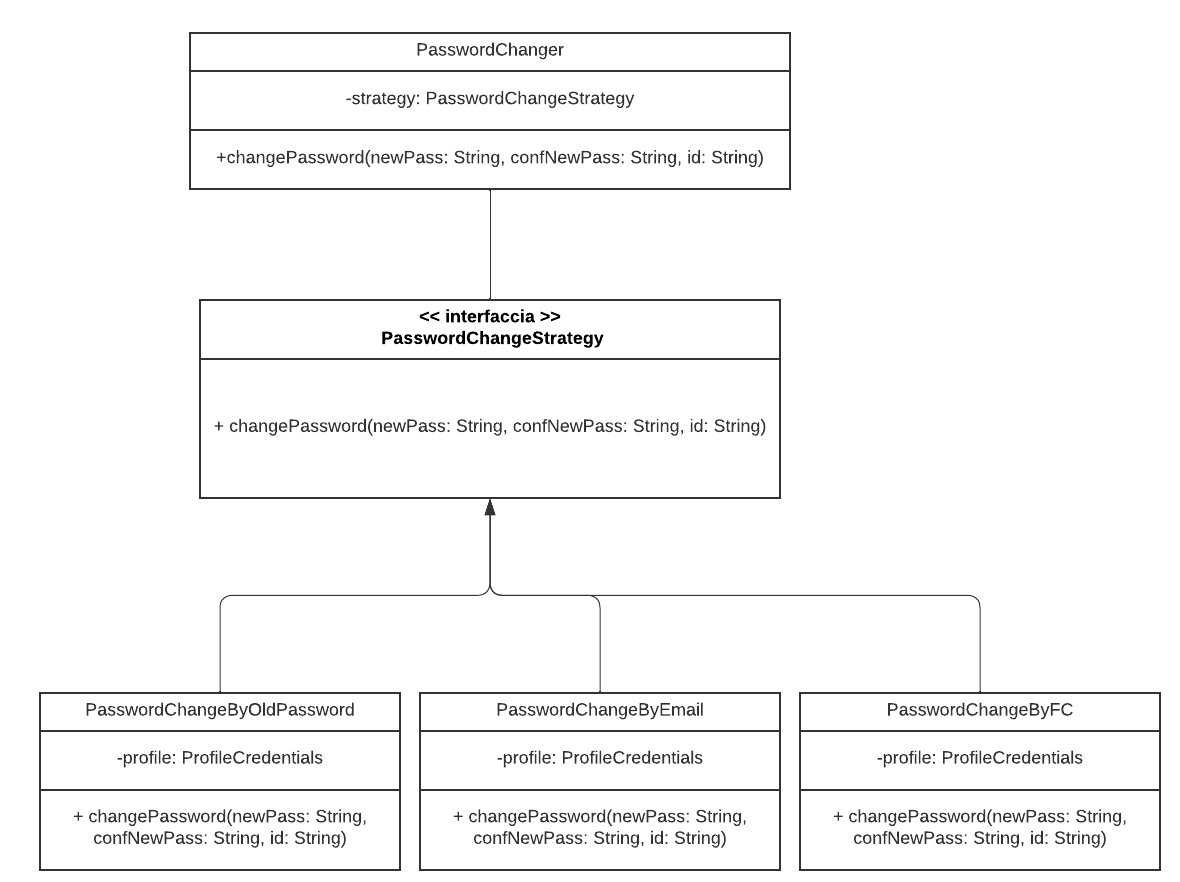
\includegraphics[width=1.2\textwidth]{img/UMLPasswordChange.png}}%
                \caption{How strategy is implemented in PasswordChange}
                \label{fig:my_label}
            \end{figure}
        
    \subsubsection{ProfileScene}
        \paragraph{Problem:}When my view was being updated it stalled the all application for about 1.5 seconds. This happened because I was retrieving all the market information while being on the JavaFx thread.
        \paragraph{Solution:}I created a Task on ControllerImpl, to be executed by a different thread, leaving the data retrieving work to Song's Observers.
            \begin{figure}[H]
                \makebox[\textwidth][c]{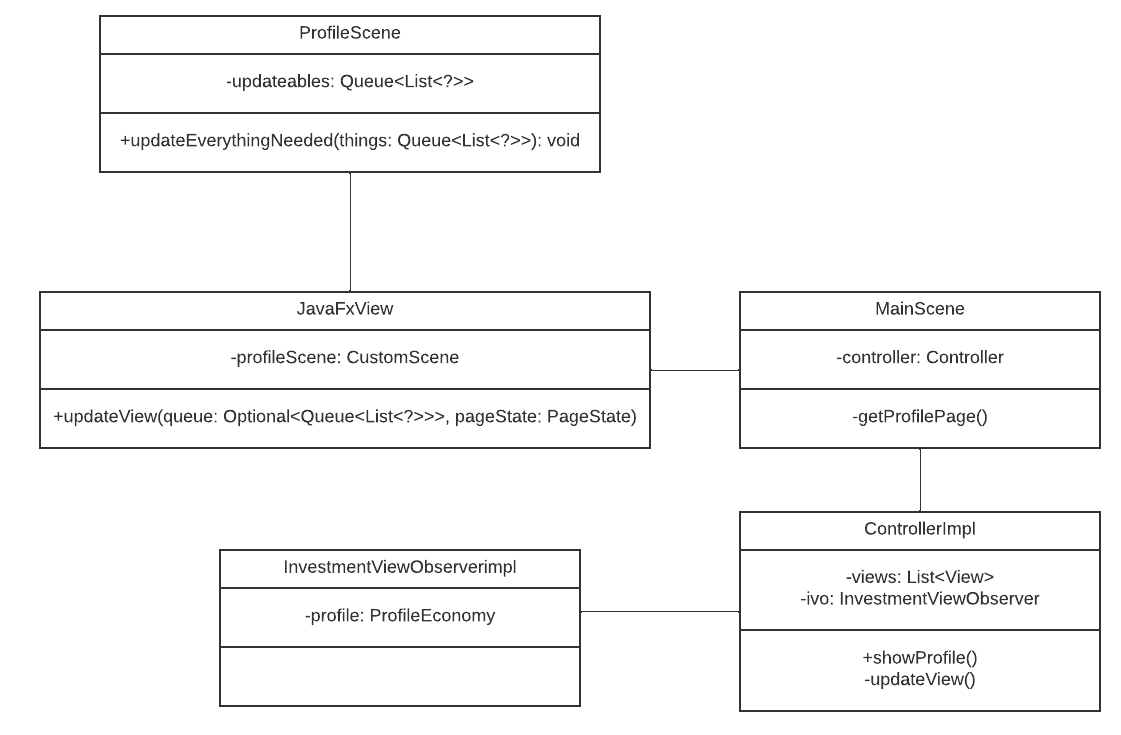
\includegraphics[width=1.2\textwidth]{img/UMLProfileScene.png}}%
                \caption{Communication between model view and controller to update ProfileScene}
                \label{fig:my_label}
            \end{figure}

\subsection{Paolo Pietrelli}

	\subsubsection{JSON}
		\paragraph{Problem:}Since I've start to think about this project,  about the profiles, the operations, I thought we need to save and manage data. 
		\paragraph{Solution:}Toghether with the team we chose to use json, in a local file, for write and read users data. For this reason I spend most of my time more than 10 days writing a class for do that easily.
		\\
		\begin{figure}[H]
                \makebox[\textwidth][c]{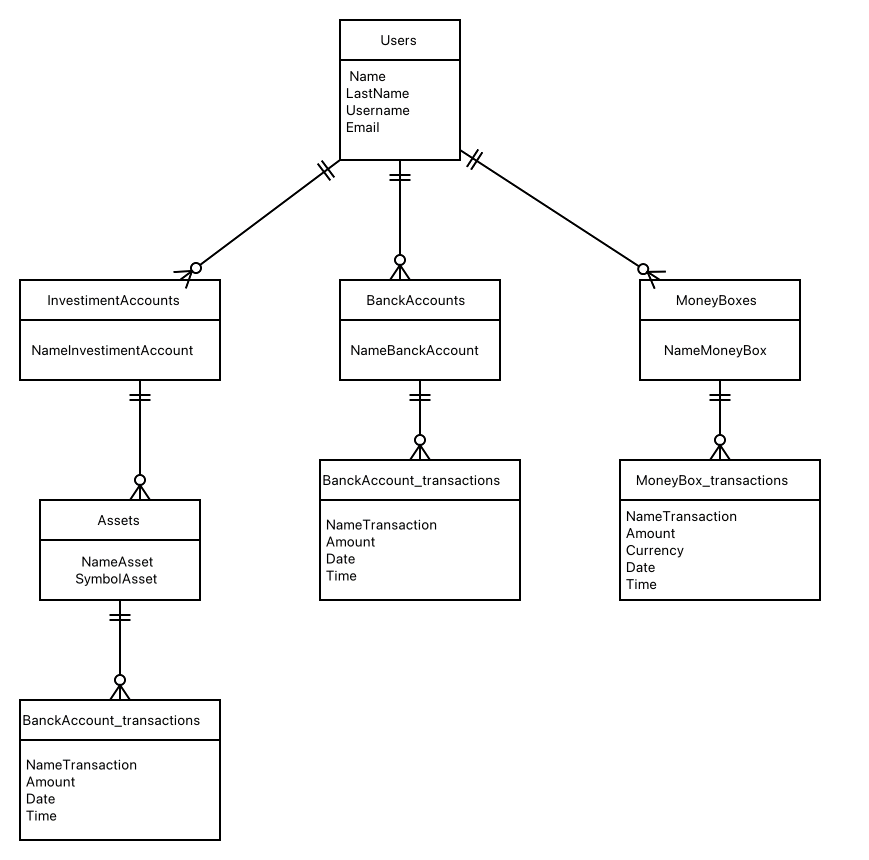
\includegraphics[width=1.2\textwidth]{img/OperationJsonFile.png}}%
                \caption{ER representation of the JSON file}
                \label{fig:my_label}
            \end{figure}
            \begin{figure}[H]
                \makebox[\textwidth][c]{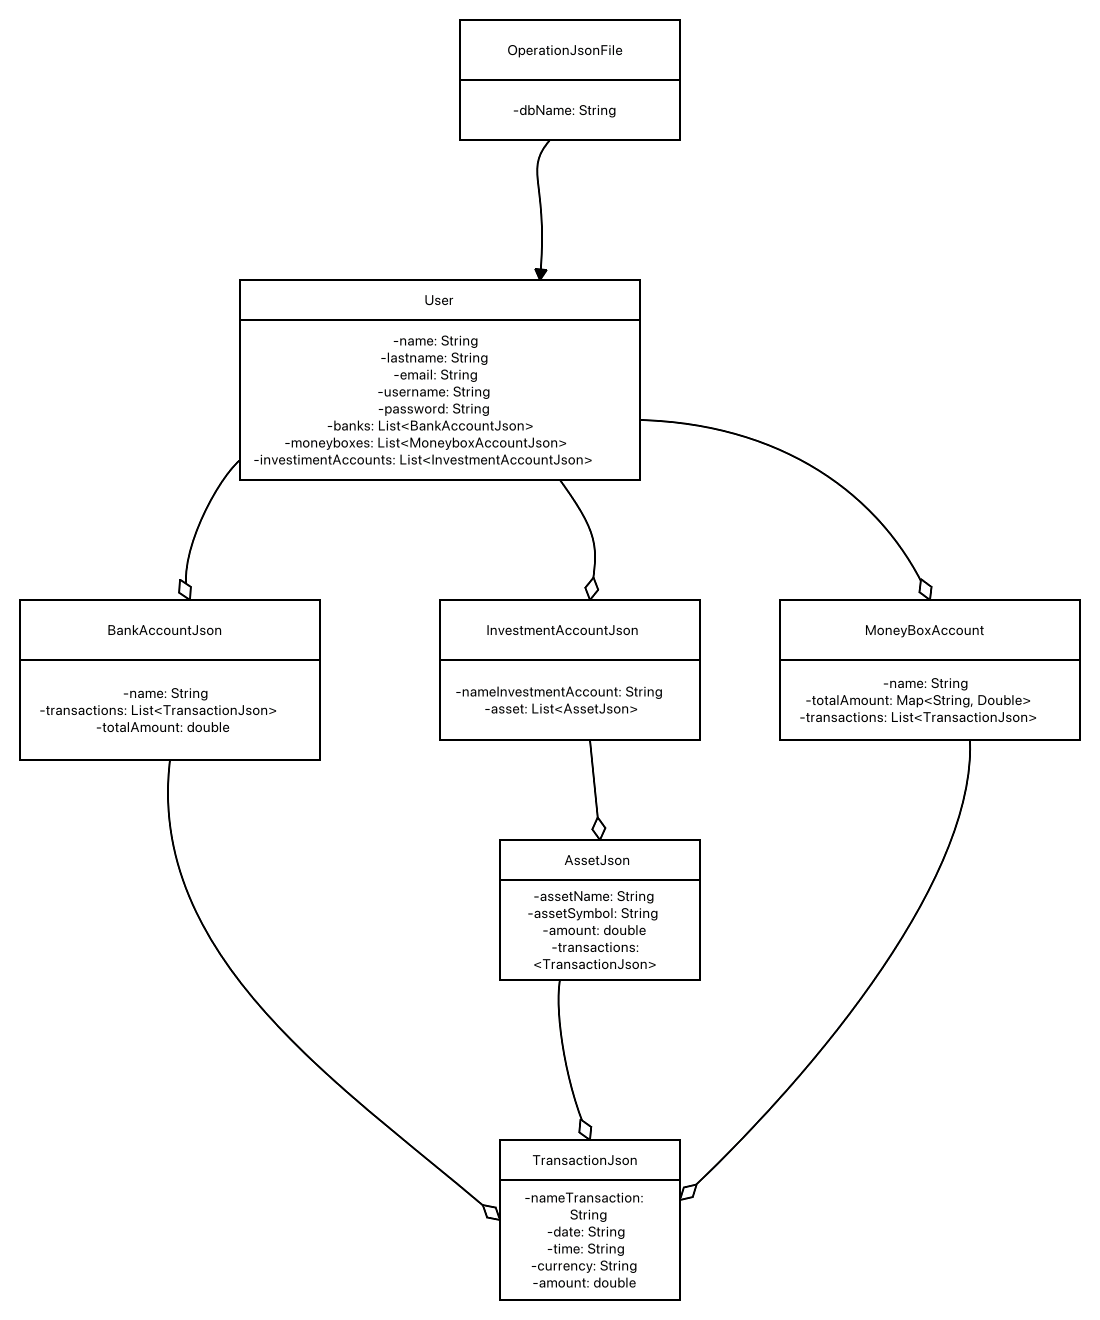
\includegraphics[width=1.2\textwidth]{img/OperationJsonFileClass (1).png}}%
                \caption{these classes are used for operate on Json file}
                \label{fig:my_label}
            \end{figure}



	\subsubsection{ExpenditureScene}
	Problem: how to show user he's transaction, and how much he spend?
	
	Solution: For solve this problem I chose to use a grafical rappresentation and focuse the view on Profit and costs;
	
	I've Project Three class TableBuilder, PieChartBuilder and LineChartBuilder, and I set their mothods for show only the transaction of the period in imput;
	
	the generality of this it been, chose for be helpfull for every member of the team, beacause the first parameter a object TransactionJson is the same for every kind of transaction in the file json.
	
	So these method are not only focused on the expenditure.
	
	 

\chapter{Sviluppo}
\section{Testing automatizzato}
For automated testing, we use the Junit 5 to test them, thanks to Gradle, we have a simple command to test all tests on the terminal, without the dependency on any editor. 

\subsection{Zhaohui Song}
I didn't spend a lot of time testing every possibility, however a minimum of tests that are deployed are:
\begin{itemize}
    \item TestAccount.java
    \item TestInvestmentAccount.java
    \item TestMarket.java
    \item TestGuiFactory.java
\end{itemize}

\subsection{Alessandro Stefani}
I tested the correct initialization of a profile and the correct change of the password inside:
\begin{itemize}
    \item TestProfile.java
\end{itemize}

\subsection{Paolo Pietrelli}
I tested my program using it and assuring me that everything was working as I expected, checking the JSON file and the output on screen.
I thought that a test could not work as I expected, because I couldn't test each method singularly, because for test the writing on json file I should then read it, and for test the reading I should before write, that mean that for test one method even the other has to work as well.

\section{Metodologia di lavoro}
\subsection{Zhaohui Song}
We have decided together that we are going to use JavaFX, from that point I have been charged to design the whole app architecture(Because I am most available on the project).
\paragraph*{Fully Independent work:}
\begin{itemize}
    \item src/model/account: \textit{Account, BaseAccount, InvestmentAccount, 
    InvestmentAccountTypeFactory, InvestmentAccountTypeFactoryImpl, NotEnoughFundsException, NotEnoughSharesException, SimpleAccount}
    \item src/model/market: \textit{Equity, EquityImpl, EquityPool, EquityPoolBasic, 
    EquityPoolAPICoinBase, EquityPoolAPITradingView, EquityPoolDecorator, 
    EquityStock, HoldingAccount, HoldingAccountImpl, Market, MarketImpl, Order, OrderImpl}.
    \item src/view: \textit{BaseScene, CustomScene, PageState}
    \item src/view/investment: \textit{InvestmentScene}
    \item src/control/investment: \textit{InvestmentViewObserver, InvestmentViewObserverimpl}
\end{itemize}

\paragraph*{Cooperated work:}
\begin{itemize}
     \item src/view: \textit{JavaFxView, GUIFactory and GUIFactoryImpl(95\%)}
     \item src/control: \textit{Controller, ControllerImpl}
     \item src/view/profile : \textit{ProfileScene (5\%)}
\end{itemize}

\subsection{Alessandro Stefani}
\paragraph*{Fully Independent work:}
\begin{itemize}
    \item main.model.profile
    \item main.view: \textit{SubscriptionPlans}
    \item main.view.profile: \textit{AddAccountView, LoginScene, PasswordChangeView, RegistrationView}
\end{itemize}
\paragraph*{Cooperated work:}
\begin{itemize}
    \item main.control: \textit{Controller, ControllerImpl}
    \item main.view: \textit{javaFxView, GUIFactory and GUIFactoryImpl(5\%)}
    \item main.view.profile: \textit{ProfileScene (95\%)}
\end{itemize}

\subsection{Paolo Pietrelli}
\paragraph*{Fully Independent work:}
\begin{itemize}
    \item main.charts
    \item main.json
    \item main.view.expenditure
    \item main.resources: \textit{utente.json}
\end{itemize}
\paragraph*{Cooperated work:}
\begin{itemize}
    \item main.control: \textit{Controller, ControllerImpl}
    \item main.view: \textit{javaFxView(2\%)}
\end{itemize}

\section{Note di sviluppo}

\subsection{Zhaohui Song}
I configured the whole project using Gradle, built dependency, including creating branches for DVCS, 
%
mainly we worked on our feature branches, I was the manager of our repository, and other members sent me code via pull request, I checked them, wrote some comments if they had programmed correctly using OOP concepts. 
%
Our main code was on the branch develop, I think it will be merged into the branch master before handing in this project.
%
Sometimes one of them commit something on the branch develop, then I had to rebase the divergence, and maintain the repository. Or maybe checkout an an file in an old hash. It was an essential tool for this project to work with more people. 

\begin{itemize}
    \item The interested feature used during development:
    \begin{itemize}
        \item Designed functions with generics, as example, the use of generics bounded (? extends Numbers) (? extends Nodes) etc..
        \item Intensive use of lambda expressions (for interface Function and predicate)
        \item Use of \texttt{Stream}, of \texttt{Optional} 
        \item Use of reflection
        \item Use of volatile variable for synchronization
        \item Use of third-party api: YahooFInance, ExecutorService, JavaFx, com.google.guava.
    \end{itemize}
\end{itemize}

\subsection*{Used code from the Internet}

I made a special package for the code of other engineers src/main/util:
\begin{itemize}
    \item AutoCompleteTextField from \url{https://gist.github.com/floralvikings/10290131} author Caleb Brinkman
    \item Pair from our class @author professori di OOP 
\end{itemize}

\subsection{Alessandro Stefani}
I unfortunately did nothing special this project:
\begin{itemize}
    \item use of lambda expressions
    \item Use of third-party api: JavaFx,
\end{itemize}

\subsection{Paolo Pietrelli}
I unfortunately needed too much time for interact with the json file, and I'm really sad my Team couldn't interact with this for the data.
And unlickily I don't know what happen the program crash and couldn't find the file json anymore.

for my code I used
\begin{itemize}
    \item third-party api: JavaFx,
    \item third-party api: Json.simple (but I also tried other library);
    \item third part class: DateTimePicker.java (https://github.com/edvin/tornadofx-controls/blob/master/src/main/java/tornadofx/control/DateTimePicker.java)
    \item third part class: NumberTextField.java (https://dzone.com/articles/javafx-numbertextfield-and)
\end{itemize}


\chapter{Commenti finali}

\section{Autovalutazione e lavori futuri}

\subsection*{Zhaohui Song}
In this project, I have been working around 5 ~ 8 hours per day for a month, I started the project on 15 July,  as today it's 16 Agost.
%
I worked in an agile way, such as writing code, then finding it redundant, then designing again, rewrite the code. 
%
It took me about 40 \% of the time on design, 40\% on coding + improving the quality, and 20\% on debugging(especially the part of threading). 
%
I tried to generalize my code as much as possible just to make this project feature-complete and reused for the future. 
%
There are too many features that can be added, such as adding a comparator to the menu, so a user can order its stocks and crypto in a preferred way, and everything you can read on readme or I mentioned above.  

\subsection*{Alessandro Stefani}
I think A really big problem in this project was the lack of planning. Although we met a couple of times to discuss the design, we only discussed it very generally, without creating any good diagram with interfaces. We also had bad communication between us and for example when me and Song confronted each other, we discovered that the idea of the architecture we had in mind differed a lot (we went for Song's idea, which was better).

\subsection*{Paolo Pietrelli}
In this project I spend many hour on research from Json to JavaFx, I think at least 40\% of my time it been spent in research, 20\% on design, 30\% on coding and only a 10\% on debugging.
I have to say that I'm agree with Alessandro we spend less time on planning and discuss together the design 

\section{Difficoltà incontrate e commenti per i docenti}
\subsection*{Zhaohui Song}

\subsection*{Problem encountered:}

Even though using the private static volatile controller is a bad solution, it works correctly with synchronization between the thread from the controller and the components on the JavaFX thread. 
I have been working on that for more than 15 hours, but still couldn't find a solution. In this case, we have multiple \textit{view}s, each of them is attached to the one controller, it wasn't something that we didn't intend to do.
Instead on the he part of controller, all \textit{view}s are accessible from a thread pool created by Executor services. 

\subsection*{Note:}
As far it's 20 August, I finally found the solution to substitute the static properties by using Application.launch(view.class, args). If I created the controller and then assign it to the views, it would be a null reference. If I create a view first, then create a controller on the JavaFX Thread. Then it wouldn't be the null reference. It's just that then I'll have to use JavaFX as the main library.
I spent like more than 20 hours just to fix this error.... I hope that it's worthy.

Thanks to prof Viroli for extending our deadline to carry out the project.
%
This course was amazing, more than I expected from what could be learning programming in java. 
%
A big thank you to every professor of this course, your lecture was easy to understand, and the lessons in the lab were so important for me to grasp these codes, along with those exercises on github.

\appendix
\chapter{Guida utente}

Once the application is launched the user will be presented with a login graphic interface.
By clicking on "Accedi" you will access the application with a DEMO account since the data retrieval
from JSON was not implemented due to bugs.
If the user wants he can also click on "Registrati" to create a brand new account with the data inserted
in the registration fields.
Once accessed the user can create an account inside the "Profilo" page, and then by clicking on "Investimenti"
is able to buy any asset on the selected account by inserting the asset's symbol (you can try AAPL, BTC-USD, AAL, TSLA ...)

\chapter{Esercitazioni di laboratorio}


\section*{Esempio}

\subsection{Zhaohui Song}

\begin{itemize}
 \item Laboratorio 06: \url{https://virtuale.unibo.it/mod/forum/discuss.php?d=87880}
 \item Laboratorio 07: \url{https://virtuale.unibo.it/mod/forum/discuss.php?d=88829}
 \item Laboratorio 08: \url{https://virtuale.unibo.it/mod/forum/discuss.php?d=89272}
 \item Laboratorio 09: \url{https://virtuale.unibo.it/mod/forum/discuss.php?d=90125}
 \item Laboratorio 10: \url{https://virtuale.unibo.it/mod/forum/discuss.php?d=91128}

\end{itemize}


\bibliographystyle{alpha}
\bibliography{13-template}

\end{document}
